\chapter{Conformational States Under Crowding}
\label{chap:WL_crowding}

\section{Experimental Motivation \label{sec:intro}}

The idealization of dilute conditions in conventional \textit{in vitro} biophysical experiments has long been recognized to ignore the important aspect of crowding. In typical cellular environments, the experimental, computational, and theoretical results have shown crowding agents to affect the stability of proteins and the rates of protein folding. The measured and predicted effects of crowding, however, are varied and seem to be dependent on both the protein and the crowders themselves. For a summary of the recent developments in the field since 2004, see the excellent review by Zhou, Rivas and Minton.\cite{zhou_macromolecular_2008} Crowding effects are still actively being explored, with most efforts focusing on the entropic effects to elucidate the response common to all crowding agents. While energetic interactions may exist between the protein and the crowding agents, a simplified yet effective treatment of a crowder is that of a steric, inert particle, affecting the entropy of the protein's conformational state according to its compactness and shape.\cite{hoppe_entropic_2009, homouz_crowded_2008}

In one limit, where the crowding particles are much larger in volume and mass than the protein, good results have been obtained by approximating the crowders through localization. Typically this is modeled as confinement between parallel plates, or in spherical or cylindrical cavities.\cite{mittal_thermodynamics_2008, wang_confinement_2009, zhou_stabilization_2001} In these approximations, the conformations that are extended beyond the confinement wall are excluded. In the other limit, where the crowders approach the size of a typical residue, the effects of excluded volume dominate. Here, not only are the extended conformal states of the protein highly perturbed, but intermediate states are also proportionally less favored to those states that are compact.\cite{minton_effect_2000}

In this chapter, we investigate the effects of crowders on the folding properties of $\beta$-sheet proteins using a lattice model. While lattice-based approaches are numerous, those that connect their results to physical experiments are less so. We are motivated by the experiments done by Gai and coworkers\cite{xu_probing_2008, mukherjee_effect_2009,du_understanding_2006} and examine our model in light of their observations. We recognize however, that simple lattice-bead models capture only a portion of the conformational entropy; typically only the gross features of the backbone are correctly modeled. To accommodate for the orientational entropy of the dihedral or $\phi$-$\psi$ angles, we introduce an Ising-like model. Each bead along the chain is associated with a binary internal state, with an interaction potential requiring the energetic contributions of two beads to have the same state. Since the correct configuration of the dihedral angles is essential for proper hydrogen-bond formations, this extra degree of freedom gives a physically motivated Hamiltonian that implicitly includes the hydrogen-bond contacts. We model the positional entropy of the backbone by projecting it onto a face-centered cubic (fcc) lattice. We use a $\Go$-like Hamiltonian to model the native connections and to ensure the existence of a unique ground state. With the conformational entropy defined we propose a model that attempts to capture the salient aspects of macro-molecular crowding using a detailed density of states (DOS) calculation. 

Once the DOS has been determined, we use the results of the scaled particle theory (SPT) to approximate the effects of crowding on several $\beta$-sheet proteins. The use of the SPT to study the conformational states of the protein folding process is, of course, not new and has been studied previously, see~\cite{mittal_dependence_2010, ping_depletion_2006, batra_effect_2009, minton_models_2005} and the references cited therein. We model the protein as right circular cylinder since the native state of $\beta$-sheets are naturally disk-like. The crowders, Ficoll 70, are modeled as sphereocylinders accounting for their observed elongation.\cite{asgeirsson_glomerular_2007, fodeke_quantitative_2010} Our treatment is unique among the previous studies in that we use the Wang-Landau algorithm to determine density of states for the positional and orientational entropies, separately. This gives us an accurate measurement of the crowding effects across the conformations of the density of states and the ability to compute thermodynamic quantities to high accuracy.

The organization of this chapter is as follows. In Section \ref{sec:methods} we introduce the Hamiltonian and the effective free energies associated with crowding and the dihedral angles. In this section, we explicitly define the cost, both enthalpically and entropically for each conformation. We demonstrate how the density of states can be factored into two terms, greatly speeding up the calculation using the Wang-Landau algorithm. We then describe the experimental results in Section \ref{sec:results} and fit our model to the experimental observations. We use the SPT to determine the effect of crowders on the thermodynamic quantities and discuss the implications. Finally, we use the results to make predictions for future experiments.

\section{Methods \label{sec:methods}}

Our protein is coarse grained to a chain of beads and projected as a self-avoiding walk onto a fcc lattice, with a `bead' representing an amino acid residue. The fcc lattice was chosen over the traditional cubic lattice to provide more degrees of freedom. Previous works have found the fcc lattice to be a more natural fit to the secondary structures of $\alpha$-helices and $\beta$-sheets.\cite{peto_generation_2007, pokarowski_minimal_2003} The choice of lattice is not arbitrary, as higher coordination numbers and different symmetries may better represent the underlying structure. For a summary on the effect of lattice choice see Pierri \textit{et al}.\cite{pierri_lattices_2008}

Two beads are considered nearest-neighbors if they are on adjacent sites on the lattice. With the underlying lattice being defined by a set of primitive vectors $\B{e}$, we define two lattice points $\mathbf{x}_i, \mathbf{x}_j$ to be nearest neighbors iff there exists a vector $\mathbf{v} \in \B{e}$ such that $\mathbf{x}_i =  \mathbf{x}_j + \mathbf{v}$. For convenience, we define the twelve lattice steps in Cartesian coordinate space $(x,y,z)$ that form the base set of a face-centered cubic lattice
\begin{equation*}
\B{e} = l
\brackets{
\begin{array}{rrrrrrrrrrrr}
1&1&1&1&0&0&0&0&-1&-1&-1&-1\\
1&-1&0&0&1&1&-1&-1&0&0&1&-1\\
0&0&1&-1&1&-1&1&-1&1&-1&0&0
\end{array}
}
\end{equation*}
%
These twelve vectors define the nearest-neighbors for a given lattice point. Here $l=3.8$\AA  \hspace{.2em} is the length scale of the lattice, which is the average spacing between two C$_\alpha$ atoms. Let the set of all backbone conformations be denoted by $\mathcal{C}$ with the vector $\mathbf{c} \in \mathcal{C}$ representing an individual conformation on the lattice. 

Our model Hamiltonian is a modification of the $\Go$-model,\cite{abe_noninteracting_1981} where the only energetic contributions are either from the attraction of the residues that are predefined native contacts or the repulsion of the nonnative ones. The $\Go$ model, primarily a model of minimal frustration, typically ignores the potential from non-native contacts. Models with the repulsive terms added,\cite{knotts_iv_entropic_2008, hoang_molecular_2000} create a frustrated energy landscape since more structural information is encoded in the Hamiltonian. In addition, the high coordination number of the fcc lattice does not always admit a unique native state for some structures without the nonnative term. We let $\GO$ be a symmetric matrix of native contacts, $\GO_{ij}=1$ iff positions $i$ and $j$ are native contacts of the protein, otherwise $\GO_{ij}=0$.  

In addition to the $\Go$-like native contacts we further require that the beads have the correct orientations. To achieve this, each bead has a binary internal state, representing the correct (or incorrect) range of values of its dihedral angles. This is similar to the ideas presented in the Mu{\~n}oz-Eaton (ME) model\cite{munoz_simple_1999} where each amino acid is allowed two internal states, folded or unfolded. While ME model has been solved exactly in a restricted form\cite{bruscolini_exact_2002} and incorporated into more extensive models,\cite{chung_temperature-dependent_2008} we exploit the fact that the ME model generates a density of internal states that is easily decoupled with the positional microstates, thus leading to more precise estimate of the thermodynamic variables. The permutations of these internal states generate an ensemble of microstates; let the set of all such state sequences be denoted $\mathcal{S}$, with the vector $\mathbf{s} \in \mathcal{S}$ representing a particular sequence of the internal states. It will be useful to refer to the total number of folded beads for a state $\sigma = \sum_{i=1}^{L} \mathbf{s}_i$, with the unfolded/folded states defined, indexed by $s_i=0 / s_i=1 $, and amino acid residue count $L$.
 
Our Hamiltonian depends on the number of native and non-native contacts of all the beads on the lattice and on their internal state
\begin{equation}
\mathcal{H}(\mathbf{c},\mathbf{s}) = 
- \sum_{i=1}^L \sum_{j=i+2}^L 
\omega_{ij} [ J_+ \mathbf{s}_i \mathbf{s}_j  \GO_{ij} - J_- (1 - \GO_{ij}) ],
\end{equation}
where $\omega_{ij}=1$ iff residues $i$ and $j$ are nearest-neighbors on the lattice and $J_{+}$, $J_{-}$ represent the strength of the $\Go$ model's native and non-native contacts, respectively. A more intuitive form can be written by counting the number of contributions from the native $\KP$ and non-native $\KM$ contacts:
\begin{align}
\label{eq:Hamiltonian}
\mathcal{H}(\mathbf{c},\mathbf{s}) &= -J_+ \KP + J_- \KM  \\ \nonumber
\KP &= \sum_{i=1}^L \sum_{j=i+2}^L \omega_{ij} \mathbf{s}_i \mathbf{s}_j  \GO_{ij} \\ \nonumber
\KM &= \sum_{i=1}^L \sum_{j=i+2}^L \omega_{ij} (1 - \GO_{ij}) 
\end{align}

There are two entropic effects incorporated into the free energy, the crowding and the dihedral angle restrictions. The free energy of a state $(\mathbf{c}, \mathbf{s})$ is
\begin{equation}
\mathcal{F}(\mathbf{c},\mathbf{s}) = \mathcal{H}(\mathbf{c},\mathbf{s})  - \beta \Delta \psi(\sigma) - \beta \Delta \mu(\mathbf{c})
\label{eq:free_energy}
.
\end{equation}
Here $\beta=1/k_B T$, $\beta \Delta \psi(\sigma)$ is the free energy term  associated with the entropy of the dihedral angle orientation and $\beta \Delta \mu(\mathbf{c})$ is an entropic cost of inserting the protein into a solution of crowders (both terms to be defined in later sections). By modeling the crowders implicitly as hard-particles there is only entropic cost for insertion, the term is truly a free energy contribution. If however, the crowder specifically interacts with the protein this contribution must be included in the Hamiltonian. The model admits three fitting parameters $(J_+, J_-, h)$, with $h$ setting the energy scale of the dihedral angle term $\beta \Delta \psi(\sigma)$. Additionally, the crowding term $\beta \Delta \mu(\mathbf{c})$, depends on the concentration and the geometry of the crowders.

The positional conformation $\mathbf{c}$ determines the number of non-native contacts $\KM$, thus we take $\Omega(\mathbf{c},\sigma, \KP)$ as the density of states. The partition function can be factored by summing up to the maximum number of native contacts $\KPMAX$:

\begin{align}
\mathcal{Z} 
    &= \sum_{\mathbf{c} \in \mathcal {C}}  \sum_{\mathbf{s} \in \mathcal {S}} 
            e^{-\beta \mathcal{F}(\mathbf{c},\mathbf{s})} \\ \notag 
    &= \sum_{\mathbf{c} \in \mathcal {C}}  \sum_{\sigma = 0}^{L} \sum_{\KP = 0}^{\KPMAX} \Big [
             \Omega(\mathbf{c},\sigma, \KP) e^{ \beta \Delta \psi(\sigma) + \beta \Delta \mu(\mathbf{c}) } 
      \sum_{\mathbf{s} \in \mathcal {S}, \Sigma {\mathbf{s}_i}=\sigma }  
            e^{-\beta \mathcal{H}(\mathbf{c},\mathbf{s})} \Big ] \notag
\end{align}


\subsection{Conformational Entropy of Dihedral Angles}

Associating an entropic cost with the correct dihedral angles is an idea that goes back to the original Zimm-Bragg (ZB) \cite{zimm_theory_1959} and Lifson-Roig (LR) models.\cite{lifson_theory_1961} These models were first used for helix-coil transitions, and later extended to include sheets.\cite{mattice_matrix_1984, hong_statistical_2008, schreck_exactly_2010} Letting each bead have an internal state, native or non-native, allows us to capture some of the detail present in more complex models, yet still retain the simplicity inherent in lattice models. It is the lack of spatial degrees of freedom that separate the ZR, LR type models from the one presented here. In our model each conformation defines a new Ising-like sub-problem, where we consider the entropy associated with the ensemble of `spins' of only the nearest neighbor contacts. 
Our model is actually the generalized variant of the spin systems, commonly referred to as the Potts model. There are two major distinctions between the Ising and Potts models; the spin directions are not necessarily restricted to two states and the strength of spins in contact are determined by an interaction matrix. We still retain the two state model, folded/unfolded, but our interaction matrix has only a single non-zero term, contributing only when both spins are in the folded state. This is evident by the $\mathbf{s}_i \mathbf{s}_j$ term in the Hamiltonian since $\mathbf{s}_i, \mathbf{s}_j \in \{0,1\}$. However, each folded residue comes at a price, the entropic cost of restricted dihedral angles for a single bead is
\begin{equation}
\beta \Delta \psi(\sigma) = h \sum_{i=1}^L \mathbf{s}_i = h \sigma
.
\end{equation}

\subsection{Reduction of State Space - Conformational Decoupling}

Since the Hamiltonian, and thus the free-energy, is a function of both positional conformations $\mathbf{c}$, and the orientational conformations  $\sigma, \, \KP$, it would seem that a calculation of the full density of states $\Omega(\mathbf{c},\sigma, \KP)$, is necessary. We will show however, that given a positional conformation, one can decouple the internal states by grouping similar conformations into isomorphic macrostates. Consider the matrix
\begin{equation}
\CHIX_{ij} (\mathbf{c}) = \GO_{ij} \omega_{ij} (\mathbf{c})
\end{equation}
of the positive energetic contributions to the Hamiltonian when one ignores the internal states. We can map this symmetric matrix to a simple, but possibly disjoint graph, $\CHIX_{ij} \rightarrow g(\mathbf{c})$, by observing that $\CHIX$ is an adjacency matrix. Let $\text{Aut}(g(\mathbf{c}))$ define the automorphism group to which $\mathbf{c}$ belongs. Each $\text{Aut}(g(\mathbf{c}))$ is a permutation group, whose members are related by mapping the vertices of the graph onto itself through permutation such that the resulting graph is isomorphic to the original. While all graphs in the same automorphism group are isomorphic to each other, we should note that not every graph is physically realizable in our lattice model due to the restriction that no two beads can occupy the same lattice site. The key to decomposing the density of states, however, is the grouping of the graphs, and hence the conformations. Each automorphism group defines a finite-graph for a spin-state system. The density of states for this finite-graph system is calculated by considering, over all possible `spins' of the system, the restricted counts of $\sigma$ and $\KP$. Since the problem of finding the internal states is identical for all members of a particular automorphism group we can decouple the density of states as
\begin{equation}
\Omega(\mathbf{c}, \sigma, \KP) = \Omega_1 (\mathbf{c}) \, \Omega_2 (\sigma, \KP; \CHIX(\mathbf{c}))
\end{equation}

As an illustrative example of the decoupling method consider a 12 bead homopolymer defined over a cubic lattice where every connection is favorable ($\GO_{ij} = 1$ if $|i-j| > 1$) in the particular conformation shown in Figure \ref{fig:Sample_homopoly_backbone}. All of the native connections, which in this case are simply all nearest neighbors, are shown in Figure \ref{fig:Sample_homopoly_connections}. Abstracting the representation to a graph in Figure \ref{fig:Sample_homopoly_graph} shows the finite system that solves the density of states over the Potts model. Usually, when solving a Potts/Ising-type system the underlying graph has a high degree of symmetry (cubic lattices or Cayley trees are common examples). For a typical graph produced by our model this symmetry is broken, forcing us to numerically compute $\Omega_2 (\sigma, \KP; \CHIX(\mathbf{c}))$. However, the number of edges in the graph determine the maximum number of favorable connections. Since this number is small, the convergence of the Wang-Landau algorithm on this portion of the DOS is rapid.
\begin{figure}[ht]
  \subfloat[][Backbone $\mathbf{c}$]{\label{fig:Sample_homopoly_backbone}
 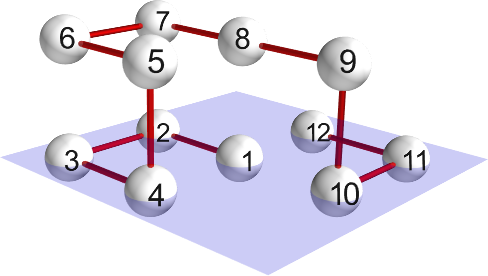
\includegraphics[width=\figurewidthTRIPLE]{WL_crowding_paper/homopoly_backbone_trim.png}}
 \subfloat[][Native Contacts $\CHIX(\mathbf{c})$]{\label{fig:Sample_homopoly_connections}
 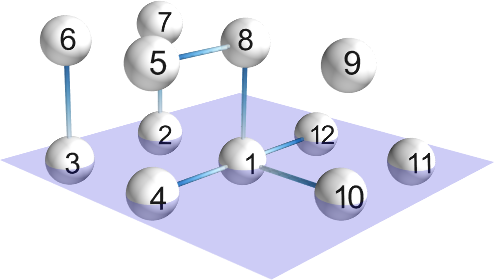
\includegraphics[width=\figurewidthTRIPLE]{WL_crowding_paper/homopoly_connections_trim.png}} \\
 \subfloat[][Connection Graph $\CHIX(\mathbf{c}) \to g(\mathbf{c})$]{\label{fig:Sample_homopoly_graph}
 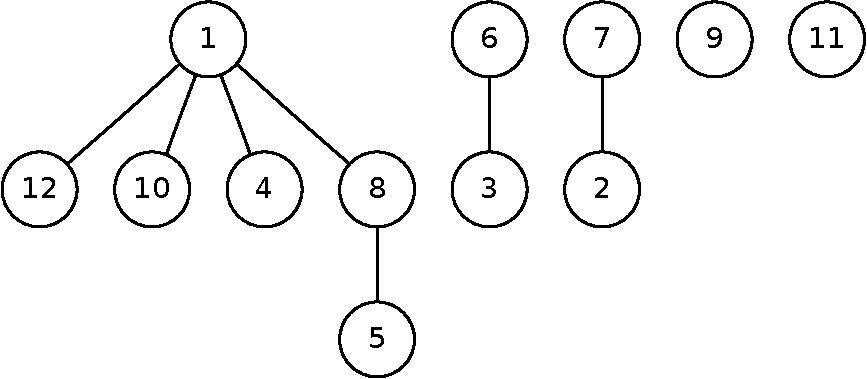
\includegraphics[width=\figurewidthSINGLE]{WL_crowding_paper/3d_example_graph-crop.pdf}}
\caption{Sample homopolymer (with all connections favorable) on a cubic lattice with (a) the backbone, and (b) the energetically favorable connections. The problem of finding the density of states for the internal conformations of each bead for this conformation is then reduced to solving the density of states of the Potts model over the graph shown in (c). Note that the labels in (c) are shown only to guide the eye, all valid permutations of the indices belong to $\text{Aut}( g(\mathbf{c}) )$ and hence define the same Potts sub-problem. The $\GO$ model in the Hamiltonian would make some of the connections in $\CHIX(\mathbf{c})$ unfavorable, further simplifying the problem. Additionally, our model is defined over a fcc lattice, while the example shown above is a cubic lattice for illustrative purposes.}
\end{figure}

In general, grouping a particular $\mathbf{c}$ to its automorphism group requires solving the graph isomorphism problem multiple times. While specialized algorithms exist,\cite{mckay_practical_1981} the computational solution is unique in its complexity class and lacks a simple invariant that definitively determines isomorphism.\cite{kaebler_graph_1993} The problem is greatly simplified if the energetic matrix $\GO$ permits only a few, highly degenerate sets of graphs. The Hamiltonian defined for $\beta$-sheets happens to be one of these favorable partitions. Since the $\beta$-sheet structure is essentially planar, moving perpendicular to the strand direction identifies a column of connections. When abstracted to a graph, the only structure possible is that of a linear chain (unary tree), whose length is limited by the number of strands. The set of conformations $\mathcal{C}$ for $\beta$-sheets create graph structures that have a high degeneracy and consequently low cardinality in the set of unique automorphism groups. Additionally, checking for graph isomorphism of linear chains is trivial since these graphs can be uniquely determined by a single number, the chain length. These two facts combined significantly speed the computation of the decoupled density of states $\Omega_1 (\mathbf{c}) \Omega_2 (\sigma, \KP; \CHIX(\mathbf{c}))$.

\subsection{Implicit Crowding Effects}
We study the effects of crowders to our protein system using the scaled particle theory. In one of the original formulations of SPT~\cite{lebowitz_scaled_1965} one calculates the work done to expand a spherical cavity of radius $R$ in a hard sphere fluid of radius $r_c$. The centers of the fluid particles are excluded from the cavity region, which implies that meaningful values of $R$ must be greater than $-r_c$. This work $W(R)$ is the configurational part of the chemical potential for a single solute particle $\Delta \mu (\mathbf{c}(R))$. The relationship between the probability of any particular configuration and the work required to create it is $P(R) = \exp( - \beta \Delta W(R))$, where $P(R)$ is the probability that there are no centers of fluid particles of radius $r_c$ in the spherical region $(R+r_c)$. If we approximate both our protein and crowders as hard-spheres, we can calculate the work required to create the proper cavity. One first calculates the probability of finding a cavity whose size can accommodate only a single spherical solute particle. This yields 
\begin{equation}
W(-r_c\!\leq R\!\leq 0) = -kT \ln(1- (4/3) \pi \eta (R+r_c)^3)
,
\end{equation} 
where $\eta$ is the number density of the solvent. One expands $W(R)$ around $R=0$ to the second order (noting that the leading term for large $R$ must be the pressure-volume term $4/3 \pi p R^3$ with $p$ as the pressure of the fluid) and obtains 
\begin{eqnarray}
\beta \Delta \mu (\mathbf{c}(R)) = &
\beta( \Delta \mu (\mathbf{c}(0)) 
 + \Delta \mu ^\prime(\mathbf{c}(0)) R \\ \nonumber &
 + \frac{1}{2} \Delta \mu  ^{\prime \prime}(\mathbf{c}(0)) R^2 
 + \frac{4}{3}\pi p R^3 )
\end{eqnarray}
These terms can be computed by the continuity of $W(R)$ and its first two derivatives at $R=0$. The pressure can be found by substituting in the exact solution of the Percus-Yevick equation, yielding a density approximation as a function of the packing fraction $\phi$. This density route is not unique among thermodynamic pathways. Expressions have been worked out for both compressibility and viral routes.\cite{chen_different_2003} Each of these pathways amount to a smoothing in the structural information of the fluid as one `turns-on' the density field. The compressibility and viral routes tend to yield better approximations to the solvation free energy, giving
\begin{eqnarray}
(\beta \Delta \mu)_\text{spherical}  &=&
\frac{\phi(-2+7\phi-11\phi^2)}{2(1-\phi)^3} 
- \ln(1-\phi) 
\\ \nonumber & &
+ \frac{18\phi^3}{(1-\phi)^3} \paren{ \frac{R}{2r_c} }
- \frac{18\phi^2(1+\phi)}{(1-\phi)^3} \paren{ \frac{R}{2r_c} } ^ 2 \nonumber
\\ \nonumber & &
+ \frac{8\phi(1+\phi+\phi^2)}{(1-\phi)^3} \paren{ \frac{R}{2r_c} } ^3 
\label{eq:SPTcrowders}
\end{eqnarray}

The above treatment by SPT assumes, however, that the cavity created is spherical, a condition that is not rigorously satisfied for the crowders nor the proteins examined in this study. The native states of the proteins studied in this work can be well approximated by a right circular cylinder, as the $\beta$-sheet structures are disk-like. Additionally our crowder, Ficoll 70, is known to have an elongated shape \cite{asgeirsson_glomerular_2007} and recent predictions\cite{fodeke_quantitative_2010} model them as sphereocylinders with diameter of 28 \AA\ and an end-to-end length of 184 \AA. The extension of SPT to work with aspherical mixtures can be expressed through the activity coefficient.\cite{boublik_statistical_1974, minton_molecular_1998} The activity coefficient $\gamma_i$ is the measure of the deviation of the ith species at the actual composition of the solution from the chemical potential of an ideal solution as given by the equation,
\begin{equation}
\label{eq:mu_i}
RT \ln{\gamma_i} \equiv \mu_i - \mu_i^{0}
\end{equation}
where $\mu_i^0$ is the chemical potential of a reference state. For hard-convex particles the non-ideality of a particular species of interest can be found by computing an expression as a function of the volume $V_i$, surface area $S_i$ and the Kihara support function $H_i$ of that species,\cite{fodeke_quantitative_2010} given by
\begin{eqnarray}
\label{eq:gamma_i}
\ln{\gamma_i} &= -\ln(1-\avg{V}) 
+ \frac{H_i \avg{S} + S_i\avg{H} + V_i\avg{1}}{1-\avg{V}} \\
&+ \frac{H_i^2 \avg{S}^2 + 2 V_i \avg{H}\avg{S}}{2(1-\avg{V})^2}
+ \frac{V_i \avg{H^2}\avg{S}^2 }{3(1-\avg{V})^3} \nonumber
,
\end{eqnarray}
where $\avg{X} \equiv \Sigma \rho_i X_i$ and $\avg{1} \equiv \Sigma \rho_i$ are the averages over the different species, with $\rho_i$ as the number density of that species. For a right circular cylinder and sphereocylinder respectively the Kihara support functions are $H_\text{\text{sphereocylin}} = r\pi/4 + L/2$ and $H_{\text{cylinder}} = r + L/4$ with $r$ as the radius and $L$ as the length of the cylindrical section. 

In the process of calculating the density of states, we can sample the conformations to determine the parameters for the activity coefficient. For each conformation of the peptide we calculate a best fit circular cylinder by pointing the axis of the cylinder along the largest principle axis of the bead positions then scale the radius and length so all beads fit inside. Using Eq. \ref{eq:mu_i} and \ref{eq:gamma_i} we can determine the free energy due to crowders in our system.


\subsection{Implementation of the Wang-Landau Method}

For a review of the Wang-Landau method and a definition of the terms see Chapter \ref{sec:wang_landau}. All of the computations carried out in this chapter took $f_0 = e^{1} \approx 2.71828$, $f_{\text{final}}= e^{-9}$, and $f_{i+1} = \sqrt{ f_{i} }$. Each time a conformation was selected, the DOS is updated along with a histogram of visits for that conformation $H(\xi)$. The factor $f$ was reduced when $H(\xi)$ was no less then $90\%$ of the average number of visits for all conformations $\avg{H}$. Once the factor $f$ had been reduced we reset the histogram of visits for all conformations, $H(\xi)=0$, and began the process again. Each conformation is still directly related to a numerical energy. By calculating the DOS for conformations we can delay the calculation of the energy. This has the advantage that multiple simulations are not required for each set of the system parameters $(J_+, J_-, h, \phi, r_c)$.

Our move set consists of pull moves, which were first defined over a cubic lattice \cite{lesh_complete_2003} and later for triangular lattice models.\cite{bockenhauer_local_2008} Pull moves are an ergodic, reversible move set that modify the positional conformations by moving the chain along a path defined by a pair of beads adjacent in chain sequence $(i, i+1)$. Since the number of moves are finite and easily computable, we can quickly determine the factors necessary for detailed balance (i.e.\ $n_A$, $n_{A \to B}$, etc).

When converged, the WL method gives a flat histogram. That is, the averaged fraction of time spent at each macrostate approaches the same constant. Here we define a macrostate as the set of all conformations with the same energy level. Not every microstate is visited during the simulation, nor would it be possible due to the exponential growth in the DOS as a function of chain length. We assume that the visits to each state are ergodic, subsequent visits to a macrostate will visit each conformation an equal number of times over long averages. This idea is reasonable when we consider detailed balance is obeyed for the Monte-Carlo simulation, and is employed by Wust and Landau.\cite{wust_versatile_2009} We exploit this observation to determine a probability distribution for a second observable as a function of the first. For instance, we can step through the conformations to compute the probability distribution of the activity coefficient for the protein in a particular conformation $\mathbf{c}$. Doing so prevents the need for a multiplicative increase in the density of states (thus speeding up the convergence of the WL algorithm), yet it still provides us with a reasonable estimate of an extended DOS $\Omega(\mathbf{c}, r_g)$.

\section{Results 
\label{sec:results}}

\subsection{Model Calibration}

Unlike $\alpha$-helices, the $\beta$-sheet motif has been difficult to study experimentally due to its propensity to aggregate. Recently there has been a spate of designed peptides that exhibit the $\beta$-sheet motif, albeit with extremely broad thermal transitions.\cite{cochran_tryptophan_2001} We consider and describe below, three experimentally designed $\beta$-sheets peptides used in this study. These designed proteins were specifically chosen to test the model against their readily available experimental measurements. 

The first peptide (sequence: \texttt{RFSEV$^D$[PG]\linebreak[0]KKFITS$^D$[PG]\linebreak[0]KTYTEV$^D$[PG]\linebreak[0]KKILQ}, nicknamed $^D$P$^D$P$^D$P) is a 28-residue chain with a natural four strand $\beta$-sheet structure. This designed peptide was studied experimentally by Xu \textit{et.\ al.\ }~\cite{xu_probing_2008} as an extension of the peptide $^D$P$^D$P-II first proposed by Gellman and co-workers.\cite{syud_influence_2003} A schematic model of the native state for the peptide is shown in Figure \ref{fig:28_residue_seq_chem_sch}. The second peptide (sequence: \texttt{RFIEV$^D$[PG]\linebreak[0]KKFITS$^D$[PG]\linebreak[0]KTYTE}, nicknamed $^D$P$^D$P) is a 20-residue chain with a natural three strand $\beta$-sheet secondary structure.\cite{hudson_measuring_2006} The final peptide (seq: \texttt{GEWTWAD[AT]\linebreak[0]KTWTWTE}, nicknamed trpzip4-m1), is a 16-residue variant of the tryptophan zippers studied by Cochran \textit{et.\ al.\ }\cite{cochran_tryptophan_2001} and later by Du \textit{et.\ al.}\cite{du_understanding_2006} Compared to the designed peptides, the stability of the tryptophan zippers is significantly higher (with a difference of approximately $\Delta G_{\text{unf}} \approx 1.0$ kcal mol$^{-1}$ at $298$ K). A schematic model of the native state for this peptide is shown in Figure \ref{fig:trpzip_residue_seq_chem_sch}.

An artifact of the fcc lattice forces the $\beta$-hairpin to be made over an odd number of lattice sites, thus we replace the Pro-Gly residues in the first two designed proteins and the Ala-Thr residues in the third peptide trpzip4-m1, with a combined residue (denoted with a square bracket, e.g..\ [PG]). The experimental measurements on these peptides have been carried out using temperature jump experiments, for details see \cite{du_understanding_2006,xu_probing_2008}.
\begin{figure}[ht]
 \subfloat[][Chemical Representation]{\label{fig:28_residue_seq_chem_sch}
 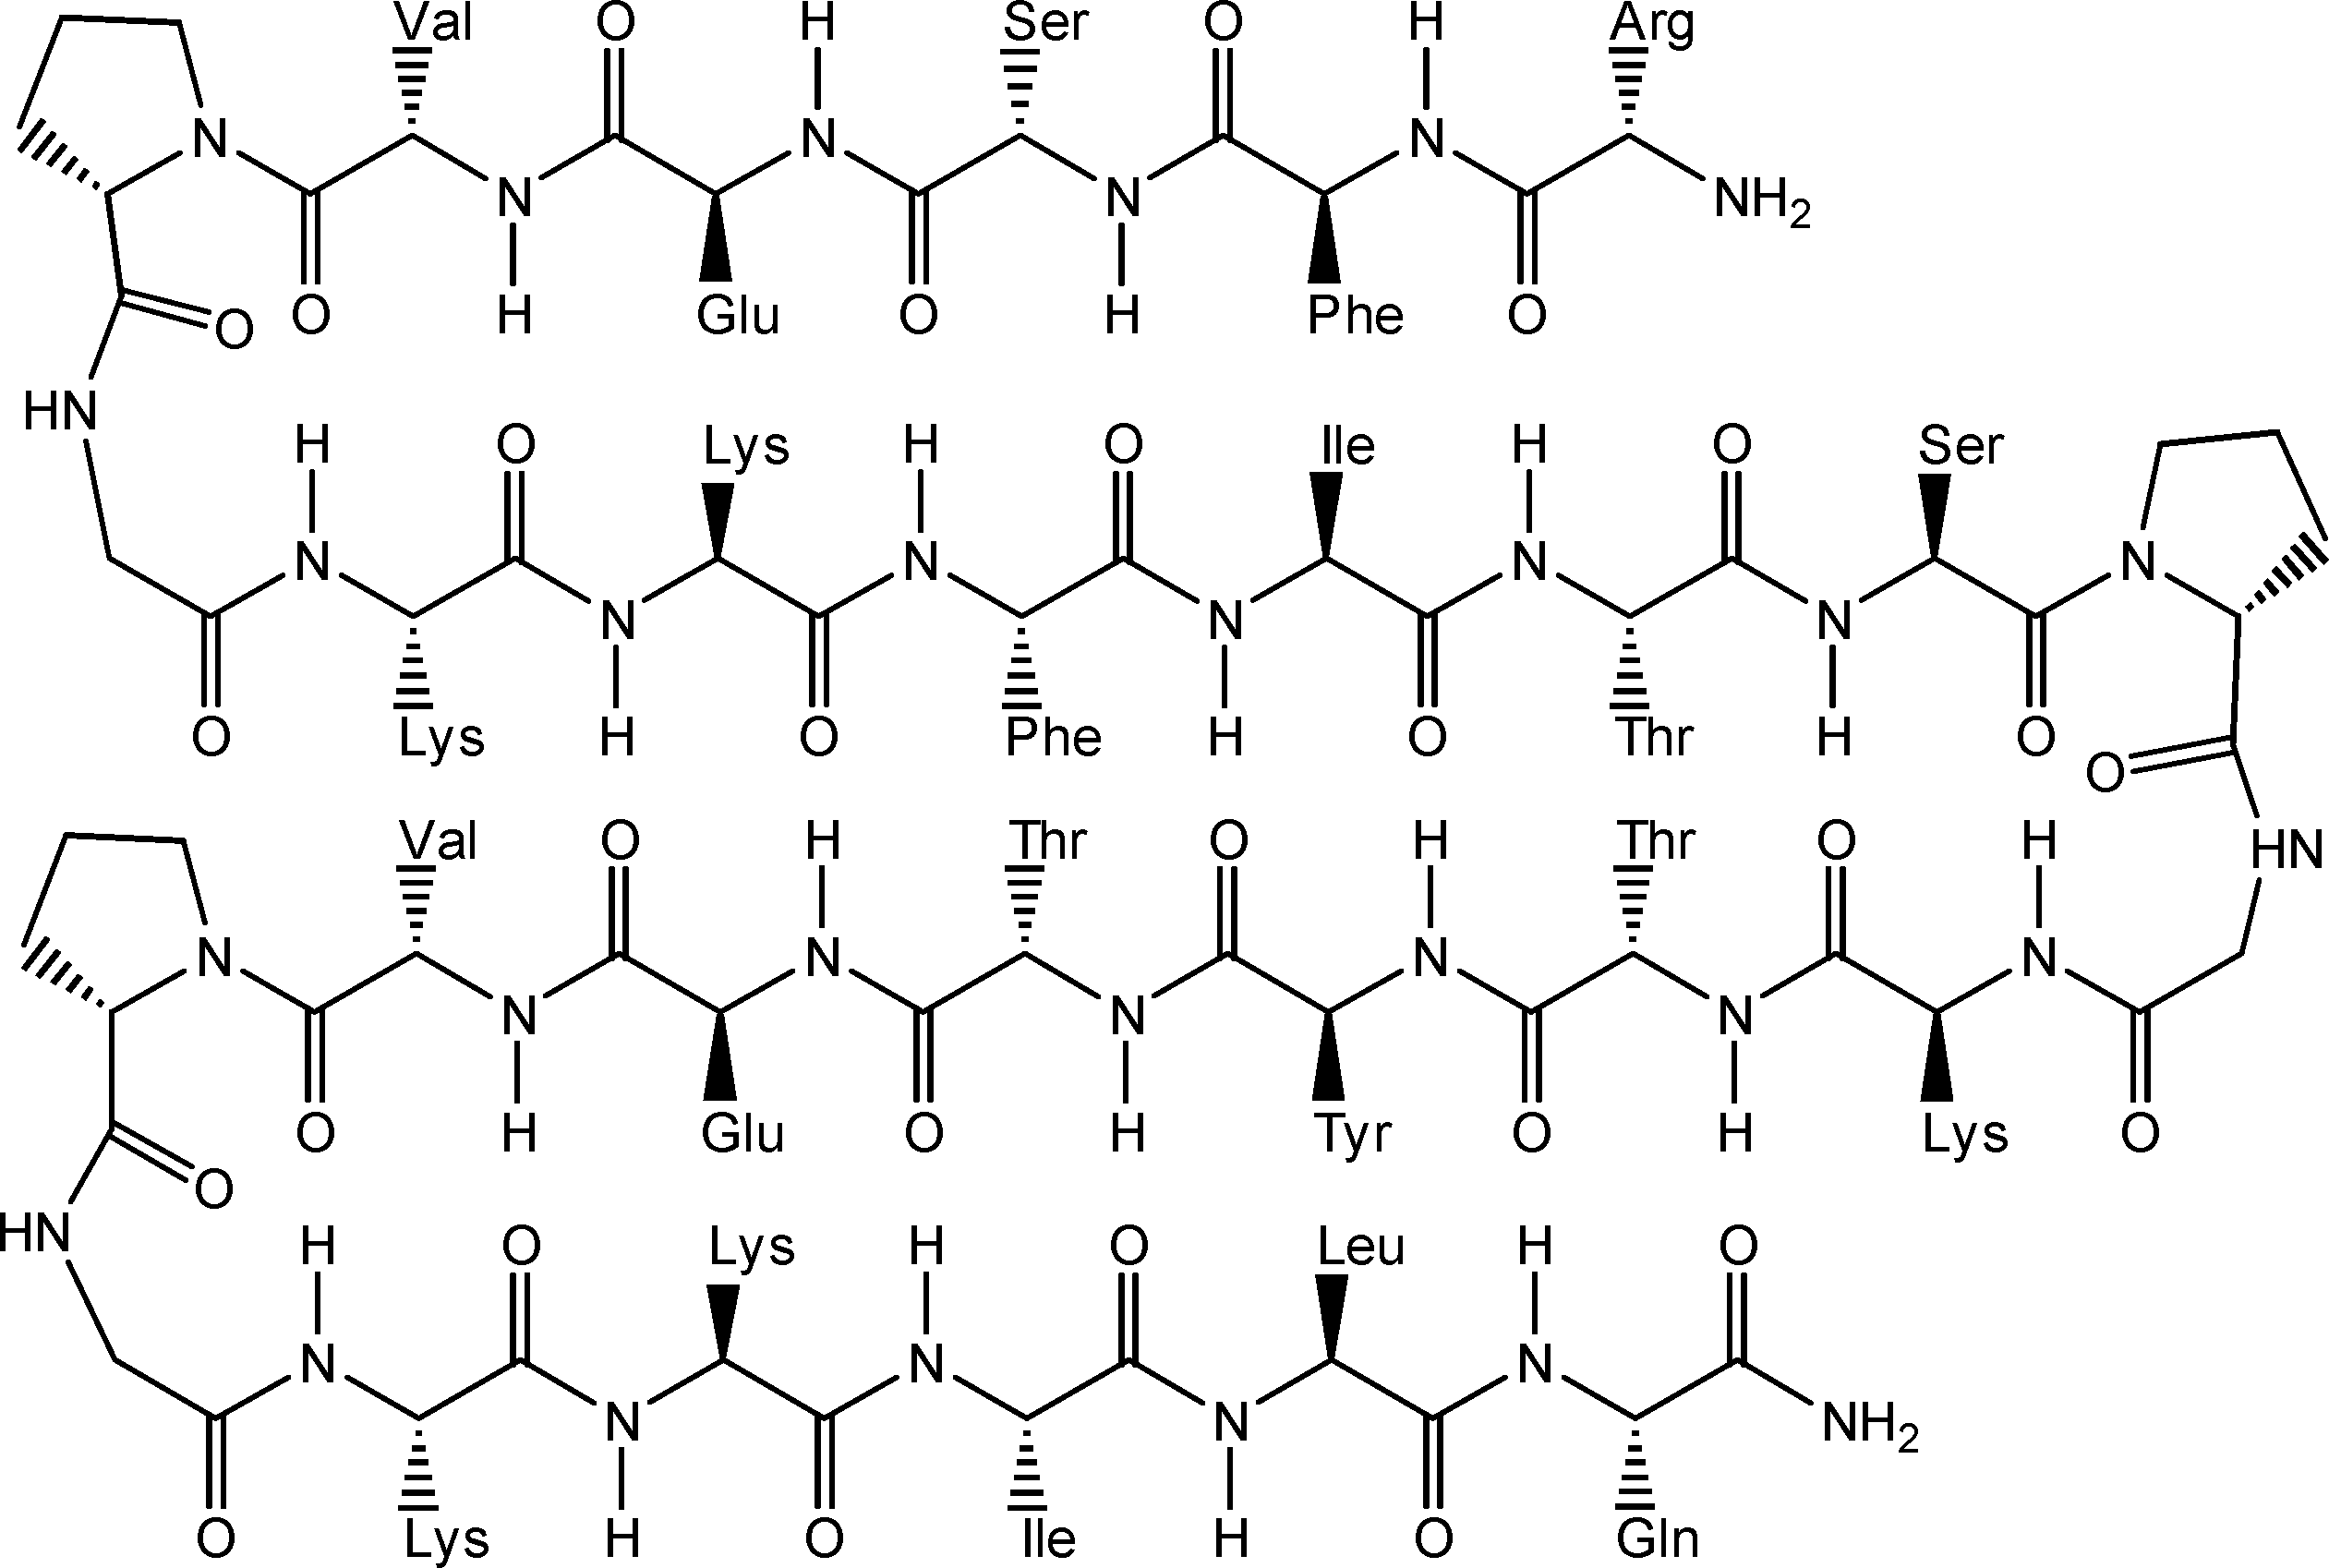
\includegraphics[width=\figurewidthSINGLE]{WL_crowding_paper/PIC_28_residue_seq_chem_sch.png}}
\caption{Native state of the peptide $^D$P$^D$P$^D$P represented schematically. The Pro-Gly amino acid residues at each end are combined to a single bead to allow for the proper turn structure on the fcc lattice. Image used with permission from Gai.\cite{xu_probing_2008}}
\end{figure}

\begin{figure}[ht]
 \subfloat[][Chemical Representation]{\label{fig:trpzip_residue_seq_chem_sch}
 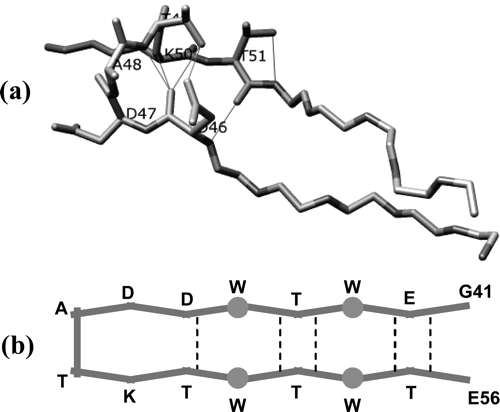
\includegraphics[width=\figurewidthSINGLE]{WL_crowding_paper/trpzipm1_du_pic.png}}
\caption{Native state of the trpzip-m1 peptide represented schematically. 
This image was generated from the NMR structure of trpzip4 (PDB code 1LE3, structure 1). The dashed lines represent the hydrogen bonds. Image used with permission from Gai.\cite{du_understanding_2006}}
\end{figure}

We use the WL method to calculate the conformations of the positional $\Omega_1 (\mathbf{c})$ and orientational $\Omega_2 (\sigma, \KP; \CHIX(\mathbf{c}))$ density of states. The model is calibrated by fitting $J_+$, $J_-$ and $h$ to the data of three experiments.\cite{xu_probing_2008, mukherjee_effect_2009,du_understanding_2006} We calculate the fraction of $\beta$-sheet contacts, observable from the experiments, by taking the expectation of $\avg{ \alpha \Theta(\alpha) }$. Here $\avg{\cdot}$ is the standard Boltzmann average, $\Theta$ the Heaviside step function and $\alpha(\mathbf{c})$ measures how close the protein is to its native state. Since the experimental data measures the fraction of $\beta$-sheet contacts (inferred from a circular dichroism measurement), we calibrated our model with physically similar observable, 
\begin{equation}
\alpha(\mathbf{c}) = (\KP-\KM)/ \KPMAX .
\end{equation}
This fraction of $\beta$-sheet contacts was used to calibrate the three free parameters. We note that without the non-native term $J_-$ in the Hamiltonian in Eq.\ (\ref{eq:Hamiltonian}) the fraction of sheet contacts would be, as usual $\avg{ \KP / \KPMAX }$.  In Figure \ref{fig:Exp_fits} we show the fits of the two proteins trpzip4-m1 and $^D$P$^D$P with the fitting parameters given in Table \ref{table:model_parameters}. The fits are quite good, encouraging us to make predictions about the system behavior as a function of crowding packing fraction. It is worth noting that the three and four stranded designed $\beta$-sheets had the best fits with $J_-=0$, implying that additional stabilization provided by the term was needed only to model trpzip4-m1. This may not be surprising when considering the larger melting points and the broad thermal transitions of the designed proteins versus that of the smaller $\beta$-hairpin peptide (listed in Table \ref{table:melting_points}).

\begin{table}
%\begin{ruledtabular}
\begin{tabular}{l|c|c|c}             
                & $h$   & $J_+$  & $J_-$  \\ \hline
Trpzip4-m1      & 9.396 & 6526.8 & 4691.6 \\
Three-stranded  & 5.103 & 2228.8 & 0.0    \\
Four-stranded   & 4.319 & 1751.3 & 0.0    \\
 \end{tabular}
 \caption{The fit parameters of the free energy (Eq. \ref{eq:free_energy}) to the model for each peptide. Here  $J_+$, $J_-$ are the strengths of the native and nonnative bonds and $h$ sets the energy scale of the dihedral angle term. }
  \label{table:model_parameters}
%\end{ruledtabular}
\end{table}

\begin{figure}[ht]
 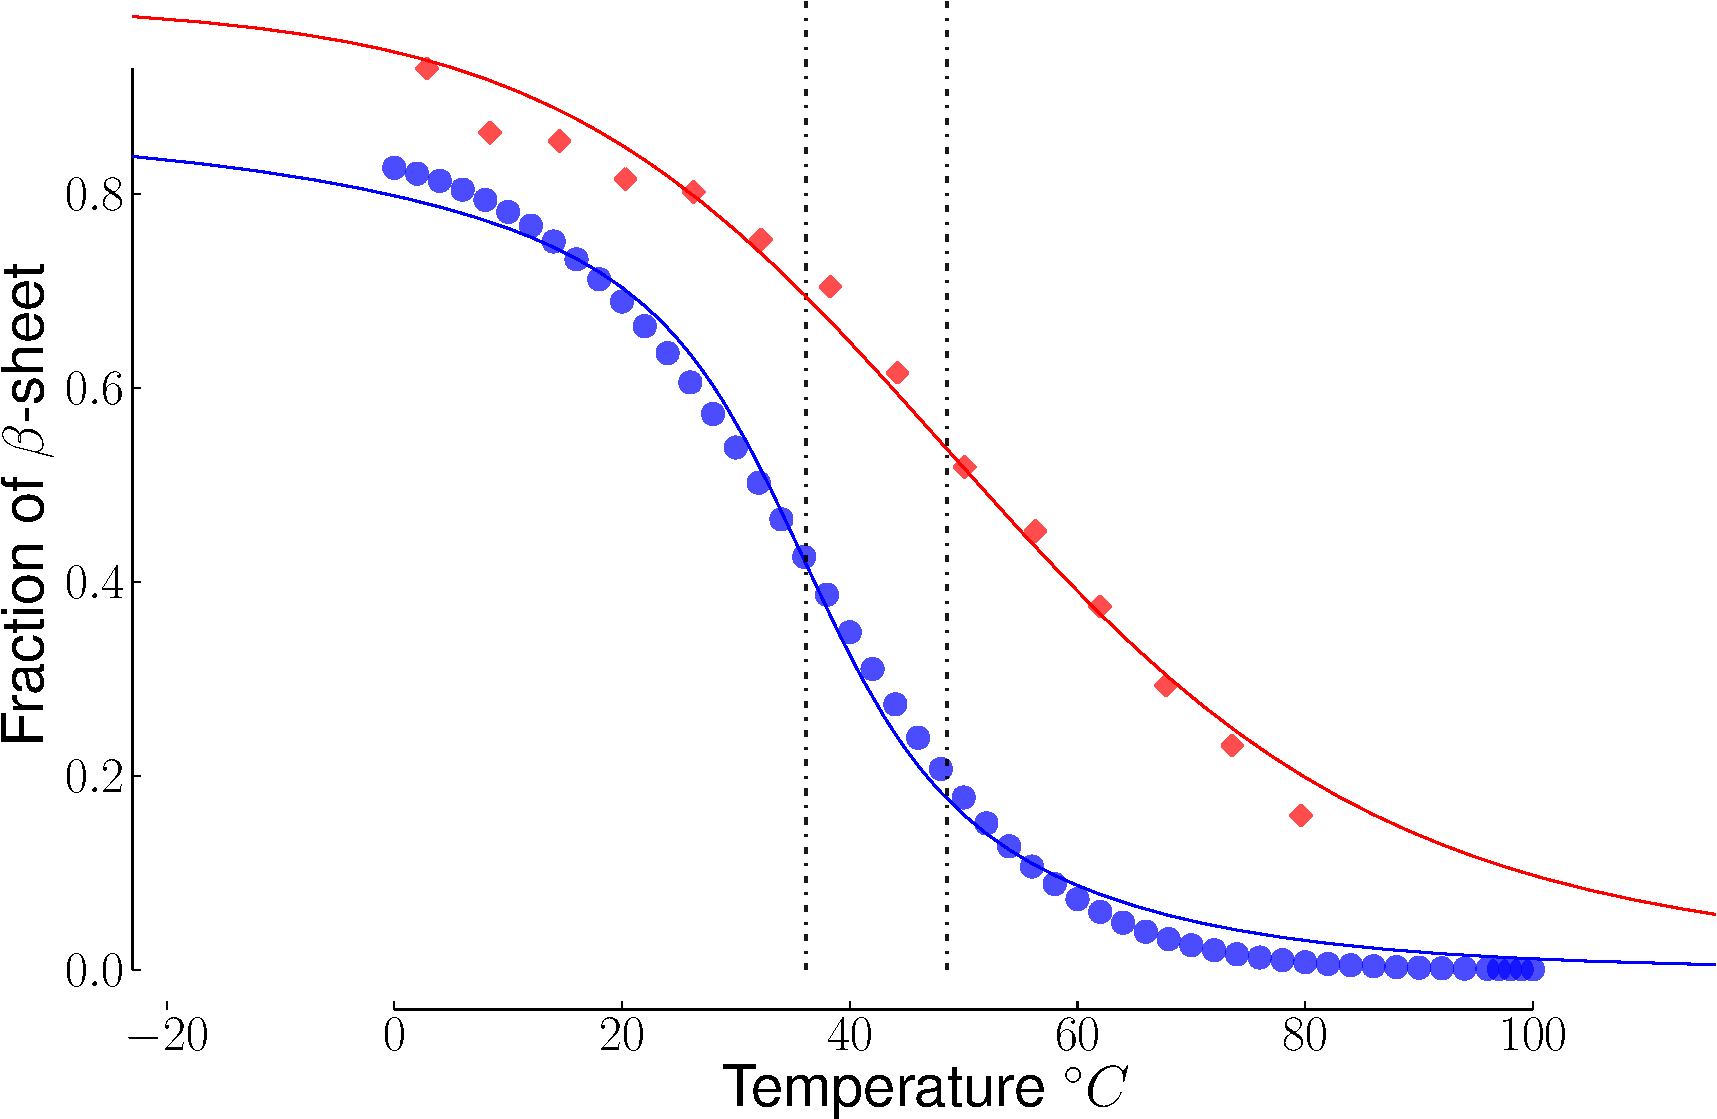
\includegraphics[width=\figurewidthSINGLE]{WL_crowding_paper/PLOT_all_experimental_fits-crop.pdf}
 \caption{Experimental data of fraction folded versus temperature for trpzip4-m1 (blue circles) and the three stranded $\beta$-sheet $^D$P$^D$P (red diamonds). Model fits are shown with dashed lines of the same color. The thin (black) vertical lines are shown to mark the critical temperatures at $36.1$ and $48.5$ $^\circ$C for three-stranded and trpzip4-m1 peptides respectively. The fit for the four stranded $\beta$-sheet $^D$P$^D$P$^D$P is similar to the three strand and is not shown for clarity.}
  \label{fig:Exp_fits}
\end{figure}

\subsection{Effects of Crowders}
In this section we use the model defined above to study the effects of crowders on peptide/protein structures and stability. For one of the peptides we have the experimental results on crowding effects to compare with. In the paper by Mukherjee \textit{et.\ al.\ }\cite{mukherjee_effect_2009} a significant change (approximately $12 ^\circ$C) in the melting point of trpzip4-m1 was observed  under crowded conditions. The crowder chosen for this experiment was Ficoll 70 (F70) at a concentration of $200$mg/ml. F70 is a compact, highly cross-linked branched co-polymer of sucrose and epichlorohydrin\cite{venturoli_ficoll_2005} with an average molecular weight of $70,000$. At $200$mg/ml, $300$mg/ml the packing fractions are approximately $\phi=0.13$ and $\phi=0.20$ respectively.\cite{lavrenko_separation_1987,dhar_structure_2010} We study the effects of crowders by considering the specific heat, $C_V(T) = \beta^2 \paren{ \avg{ E^2 } - \avg{E}^2}$ and note that in all cases, we observe only a single maxima. We identify this maxima as the melting temperature $T_C$ (alternatively, $\pfrac{C_V}{T} | _ {T_C} = 0$). 

Heat capacity as a function of temperature for trpzip4-m1 is shown in Figure \ref{fig:trpzip_CV_plot} while the melting points for all peptides listed in Table \ref{table:melting_points}.  As expected, trpzip4-m1 displays crowding enhanced stability with the change of critical temperature $\Delta T_c=[1.03, 1.65] ^\circ C$ at packing fractions $\phi=[0.13, 0.20]$ respectively. However, the three and four stranded $\beta$-sheets exhibit a slight decrease in their critical temperatures with $\phi$, indicating an entropically based \textit{instability} caused by the crowders. 
\begin{figure}[ht]
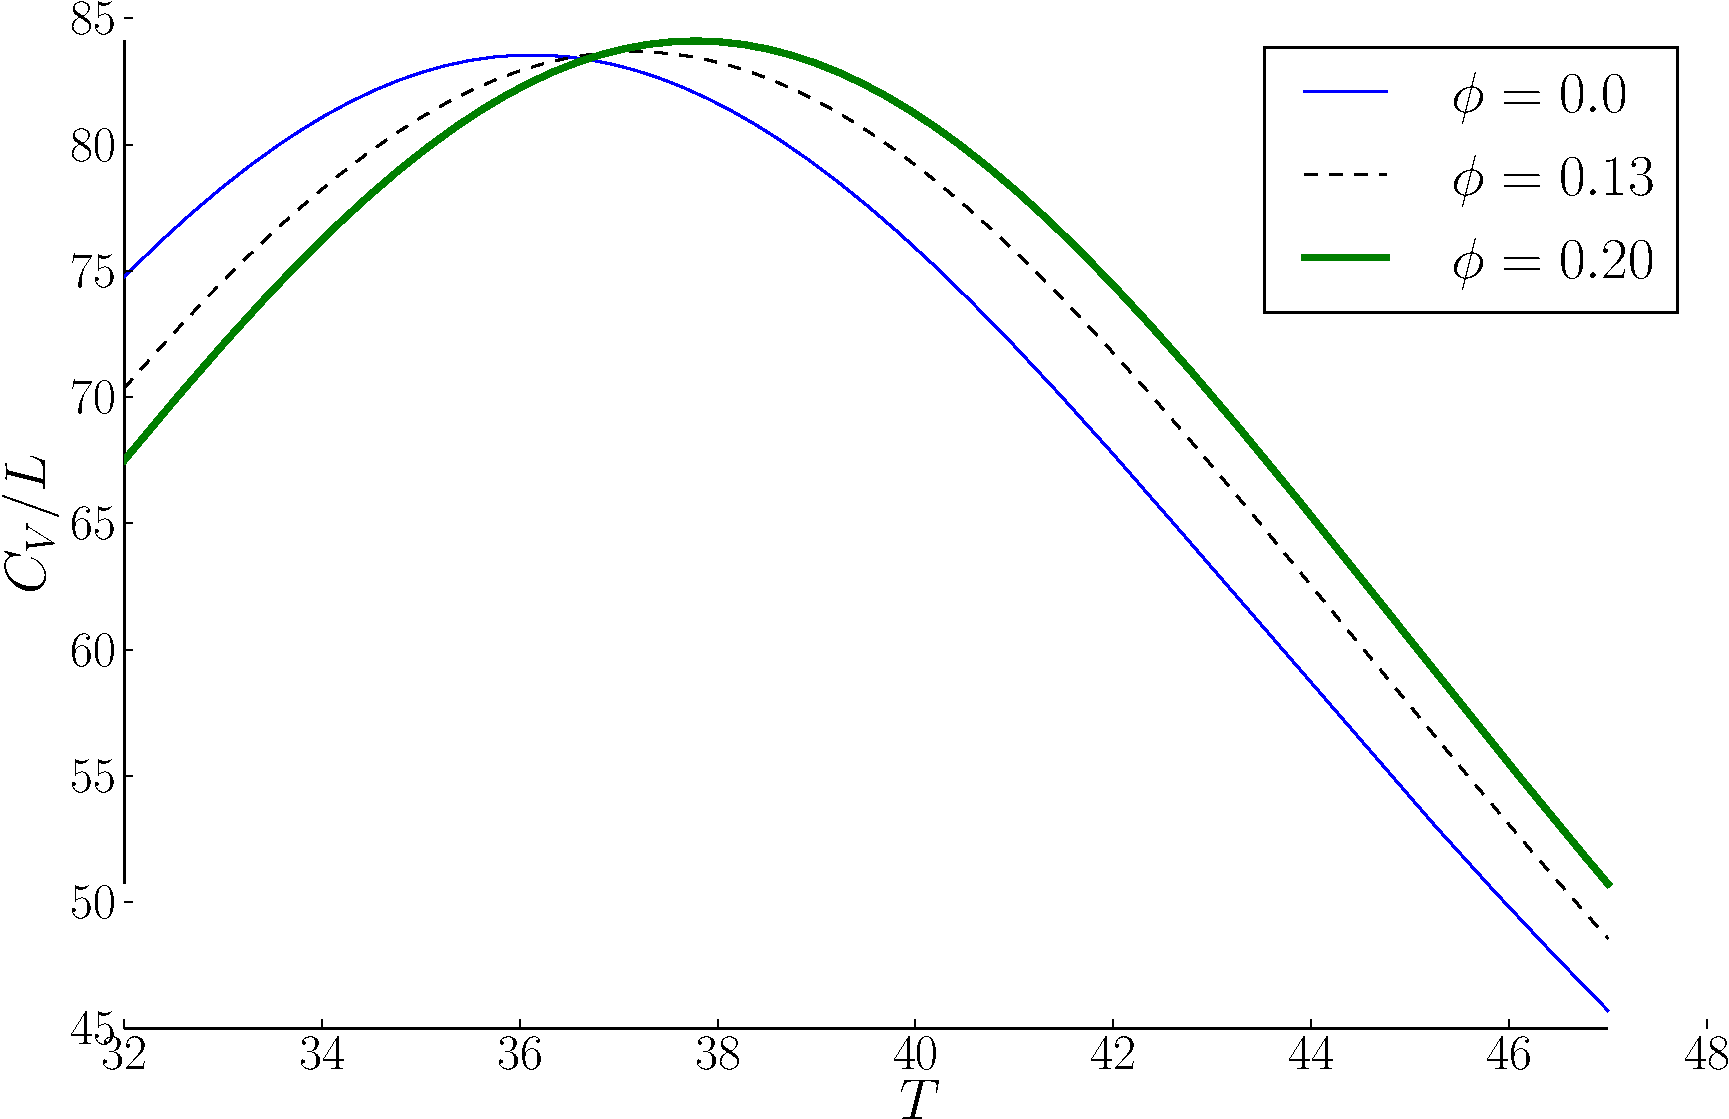
\includegraphics[width=\figurewidthSINGLE]{WL_crowding_paper/PLOT_trpzip_CV-crop.pdf}
\caption{Specific heat per residue count for the protein trpzip4-m1 in the presence of crowders.}
\label{fig:trpzip_CV_plot}
\end{figure}

%(309.12030531285251, 1) (310.14776783118413, 1) (310.77520920698208,    1.64
%(321.48930681998843, 1) (321.22525050654366, 1) (321.10529390266174,   -0.39
%(322.18103000528168, 1) (322.00889196768372, 1) (321.9355172255685,    -0.24 

\begin{table}
%\begin{ruledtabular}
\begin{tabular}{l|c|c|c|c|c}             
                          & Experimental    & $\phi=0$ & 0.13  & 0.20  \\ \hline
Trpzip4-m1                & $32.1 \pm 0.9$  & 36.12    & 37.15 & 37.76 \\
Three-stranded            & $52.6 \pm 0.4$  & 48.49    & 48.23 & 48.10 \\
Four-stranded             & $50.5 \pm 0.8$  & 49.18    & 49.01 & 48.94 \\
\end{tabular}
\caption{List of the experimental and model melting points (given in $^\circ C$) for each peptide. The experimental melting points are taken from \cite{xu_probing_2008, mukherjee_effect_2009, du_understanding_2006} in a dilute solution without crowders. The calculated melting points from the model are given at the listed values of the packing fraction. Not shown is the experimental value of trpzip4-m1 in the Ficoll 70 solution of $200$ mg/ml with $T_C=44.0 \pm 0.2$ $^\circ$C.}
\label{table:melting_points}
%\end{ruledtabular}
\end{table}

The native state for the three and four stranded $\beta$-sheets are highly aspherical. When considering the entropic effects of crowders, the system prefers compact conformations that minimize the excluded volume effect. As a consequence of this, the native state ceases to be the minimum free energy conformation at large enough $\phi$. Crowding-induced conformational change of the native state has been observed experimentally in a recent work by Dhar \textit{et.\ al.\ }\cite{dhar_structure_2010} who studied phosphoglycerate kinase (PGK) with the same crowders as our simulations (Ficoll 70). In this study, the conformational states were changed dramatically with crowders; an optimal non-zero packing fraction of crowders was found to increase the protein's activity. In our simulation, there was no shift to a new distinct native state at higher crowding concentrations. Rather, we observed a gradual shift towards more compact conformations at the expense of breaking energetically favored bonds, a general collapse of the $\beta$-sheet. As an example of the native conformation, which is enthalpically favored, versus an entropically favored one see Figure \ref{fig:sample_states}. Previous studies that showed crowding enhanced stability often dealt with globular wild-type proteins, whose natural environment required them to operate in crowded conditions. In contrast to the PGK study, the two larger peptides in our study were not wild-type, rather they were designed and studied because of the fact that they folded into beta-like conformations at realistic temperatures without aggregation. This suggests further experimentation on the designed peptides to determine if the destabilization of the native state against those of the unfolded and intermediate states under crowded conditions can be observed experimentally. 
\begin{figure}[ht]
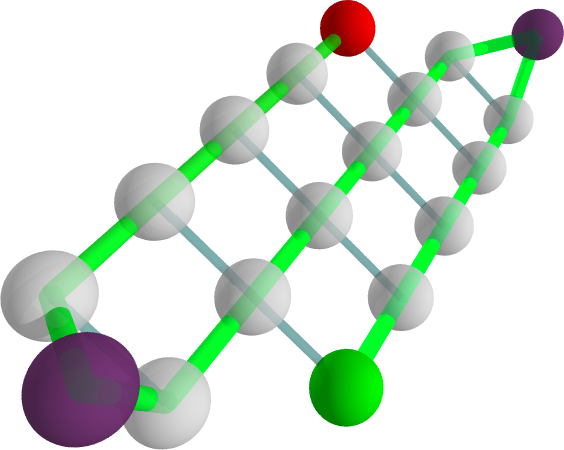
\includegraphics[width=5cm]{WL_crowding_paper/samplepic1.png} 
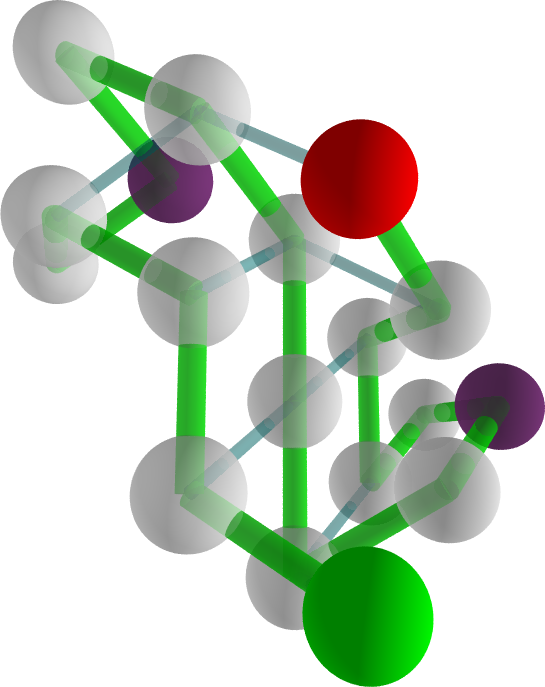
\includegraphics[width=5cm]{WL_crowding_paper/samplepic2.png}
\caption{Example of native state (top) and intermediate state (bottom) of the three-stranded peptide. The top state has ten bonds (shown as thin blue lines) while the bottom has eight bonds, making the native state favored energetically. However the ratio of activity coefficients $\ln \gamma_1 / \ln \gamma_2$ is $1.13$ at 200 mg/ml ($\phi = 0.13$) favors the eight bond structure due to the entropic crowding effects. The C and N terminus marked with red and green beads respectively and the combined Pro-Gly amino acid residues are purple beads.}
\label{fig:sample_states}
\end{figure}


In order to assess the effect on the conformational states we examine the Boltzmann averaged excess chemical potential from the native state as a function of temperature and $\phi$ 
\begin{equation}
\label{eq:d_mu}
\beta \avg{ \Delta \mu_{\text{ex}}(T) }  =  
\avg{ \ln{\gamma_i} - \ln{\gamma_N} }
.
\end{equation}
Figure \ref{fig:trpzip_chem_change_plot} of this free energy term for trpzip4-m1 illuminates several interesting structural features from an ensemble perspective. At large temperatures we see that this excess chemical potential approaches a constant, proportional to the change in the unfolded states due to the crowders. Conversely, at very low temperatures crowders have no effect on the only viable conformation, the native state. Near the folding transition temperature, the effect is large and non-linear.

\begin{figure}[ht]
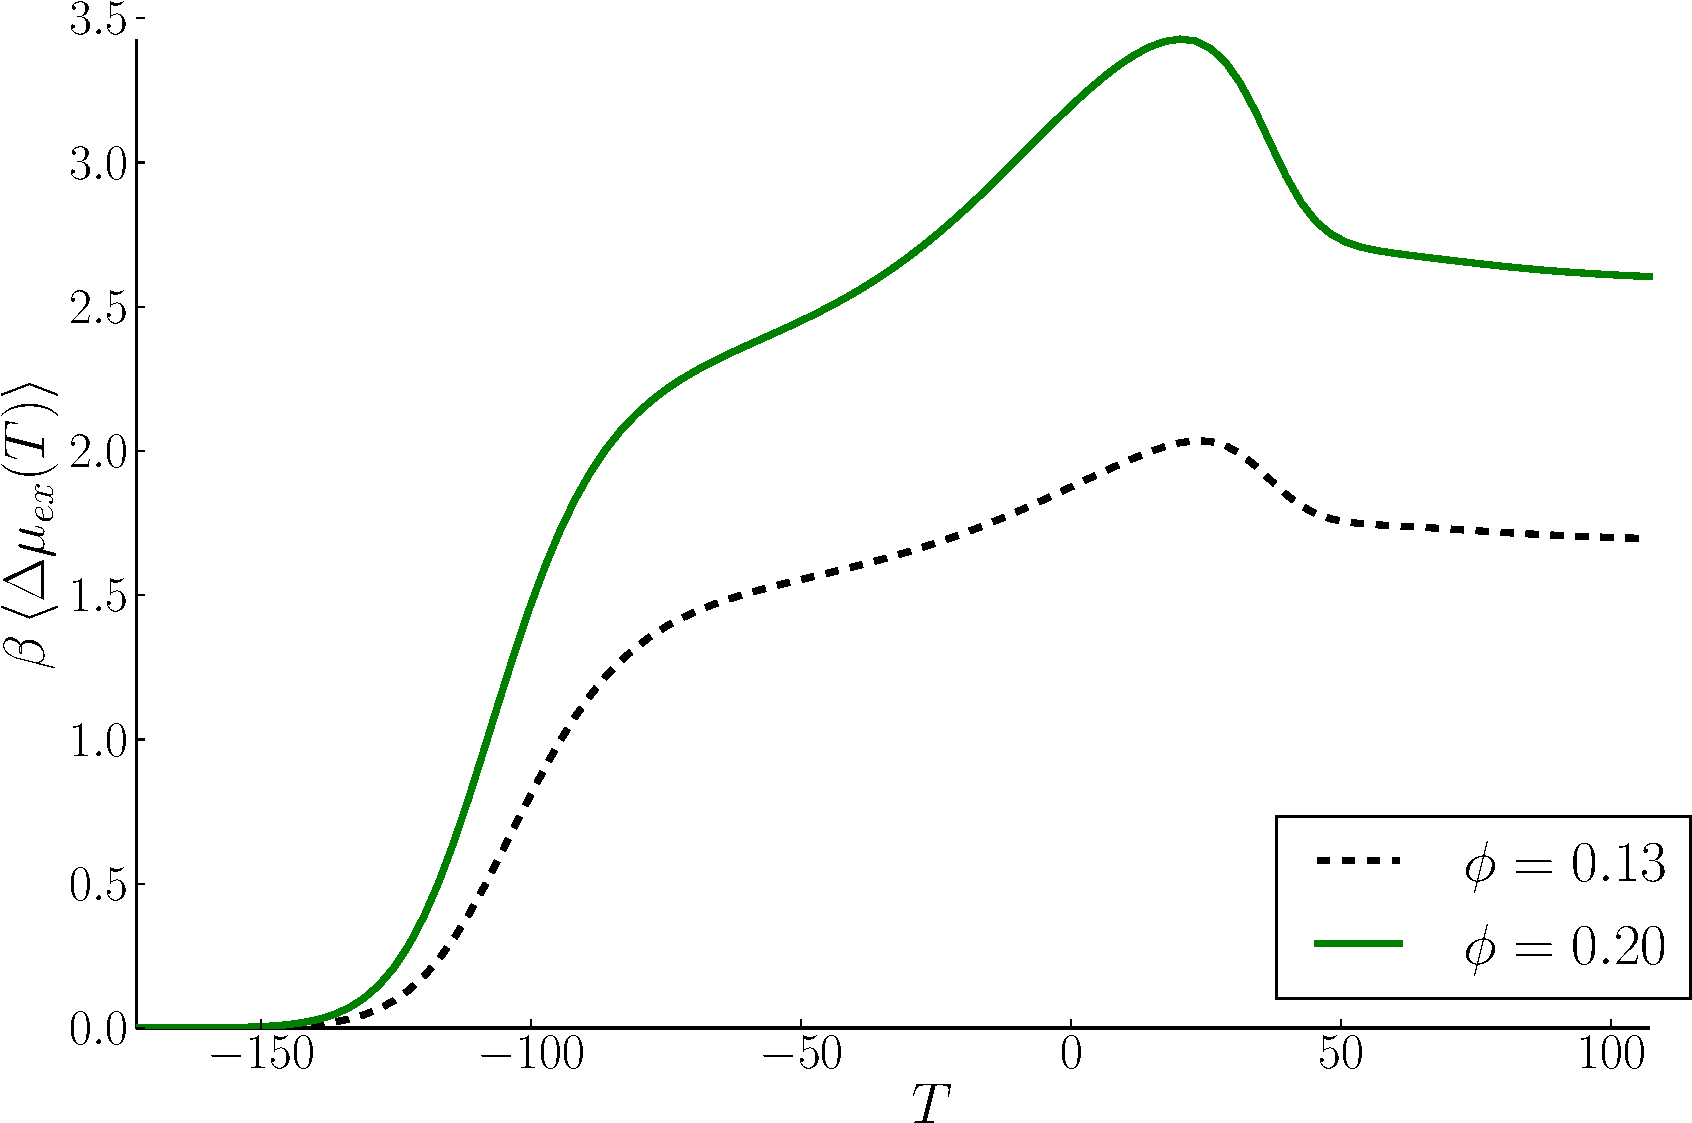
\includegraphics[width=\figurewidthSINGLE]{WL_crowding_paper/PLOT_trpzip_change_chem_pot-crop.pdf}
\caption{Excess chemical potential (defined in Eq. \ref{eq:d_mu}) for the protein trpzip4-m1 in the presence of crowders.}
\label{fig:trpzip_chem_change_plot}
\end{figure}



\section{Discussion \label{sec:conclusion}}
In this chapter we developed a coarse-graining model for proteins by combining the Ising-like state information of the dihedral angles of the modeled $\beta$-sheet structures with a fcc lattice model. The density of states has a favorable decoupling which enabled us to use the Wang-Landau method to determine the partition function accurately, giving excellent quantitative agreement with previous \textit{in vitro} experiments. Using our model and the predictions of SPT we found crowding-induced stability, in qualitative agreement with experiment for the smaller peptide, trpzip4-m1. The effect predicted by this model by showed a modest change of about $\approx 1^\circ$C, in contrast the the large change observed in the experiments of Mukherjee.\cite{mukherjee_effect_2009} We note however, that these coarse-grained models are approximations and selectively ignore various interactions. The study presented here is an entropic one. If the crowders have enthalpic interactions with the peptide, then these predicted effects will be incomplete. We attribute this underestimation to effects that cannot be explained by excluded volume effects alone.

We found that that the model predicted instability for the designed three- and four-stranded $\beta$-sheet peptides. This is consistent with the observation that their native state does not minimize excluded volume effects (it is disk-like rather then globular). This observation alone however, is not sufficient to predict of crowding based instability. Even if the native state is non-ideal, one has to consider the entire ensemble of states as a whole. This was possible using the Wang-Landau method which allowed us to accurately determine the density of states under the constraints of our model.  

The extension of the $\Go$-like contact map to a finite graph presented here is not limited to the $\beta$-sheet motif. This entropic model of conformational states can be extended to $\alpha$-helices or a mixture of secondary structures, as long as the contact graph structure can be decomposed into simple degenerate forms. 

\begin{comment}

\section{-= Working =-}

Given two conformations, $\mathbf{c}_1, \mathbf{c}_2$ and their respective density of states, we may want to determine when and under what conditions, the two states are equiproportional. That is, we would like to solve the free energy equation:
\begin{align}
\frac{ \mathcal{F}_1(\mathbf{c}_1)} {\mathcal{F}(\mathbf{c}_2) } &= 1 \\
\frac{ g_1 \exp( \beta( \sigma_1 h - k_1 J_+ + \Delta \mu(\mathbf{c}_1))  )  }
     {g_2 \exp( \beta( \sigma_2 h - k_2 J_+ + \Delta \mu(\mathbf{c}_2))  ) } &= 1 \nonumber 
\end{align}
This can be rearranged to give:
\begin{align}
\label{eq:criticalphiA}
\Delta \mu(\mathbf{c}_{12}))
&= \Delta \mu(\mathbf{c}_1)) - \Delta \mu(\mathbf{c}_1))  \\
&= \ln \paren{ \frac{g_1}{g_2} } + \beta h(\sigma_1-\sigma_2) - \beta J( k_1 - k_2) \nonumber
\end{align}

Using the values for $\Delta \mu(\mathbf{c}_12))$ from equation (\ref{eq:SPTcrowders}) we get:
\begin{align}
\label{eq:criticalphiB}
\Delta \mu(\mathbf{c}_{12}))
&= \frac{18\phi^3}{(1-\phi)^3} \paren{ \frac{R_1 - R_2}{2 r_c} } \\
&- \frac{18\phi^2(1+\phi)}{(1-\phi)^3} \paren{ \frac{R_1 ^2 - R_2 ^2}{4r_c^2} } \nonumber \\
&+ \frac{8\phi(1+\phi+\phi^2)}{(1-\phi)^3} \paren{ \frac{R_1 ^3 - R_2 ^3}{8 r_c ^3} } \nonumber
\end{align}

Combining equations (\ref{eq:criticalphiA}, and \ref{eq:criticalphiB}), gives us a polynomial in $\phi$ of third degree. If we hold the other parameters fixed (e\.g.\ $\beta, r_c$, \ldots) and let the native state correspond to $\mathbf{c}_2$, can numerically solve for this critical $\phi_c$. This $\phi_c$, if it exists and is physical,  corresponds to a switching point in the system. At this crowding concentration, the energetically favored native state is less likely to be found then a higher energy, but more compact conformation.
\end{comment}
